%!TEX root = ../template.tex
%%%%%%%%%%%%%%%%%%%%%%%%%%%%%%%%%%%%%%%%%%%%%%%%%%%%%%%%%%%%%%%%%%%%
%% chapter5_PrototypingPerf.tex
%% NOVA thesis document file
%%
%% Chapter with the Prototyping and Performance Evaluation Results part
%%%%%%%%%%%%%%%%%%%%%%%%%%%%%%%%%%%%%%%%%%%%%%%%%%%%%%%%%%%%%%%%%%%%

\typeout{NT FILE chapter5_PrototypingPerf.tex}

\chapter{Prototyping and Performance Evaluation Results}\label{cha:chapter5_PrototypingPerf}

%So neste capitulo e que se deve descrever a operacao do circuito.
Upon completion of the circuit design phase, the next step starts to dictate the physical shape of the prototype.

\section{PCB Layout}\label{sec:51_PCBlayout} % se calhar tiro "Design"
%provavelmente este capitulo deve ficar no final do Chapter 4, porque layout também é hardware design

\subsection{Footprint Assignment and Placement}\label{sec:511_Placement}

Once every component symbol in the schematics is correctly referenced and the electrical rules check reports no errors nor warnings, KiCad provides a footprint assignment tool, to attribute the desired footprints to the project's parts. Since the new beRTK\textsuperscript{\textregistered} circuit is based around fourteen main ICs and modules, selecting the correct footprints for each of these was the starting point for the layout phase. For that, datasheets for ICs and modules usually feature a section dedicated to presenting the recommended footprint for their component. This facilitates designers' work, as KiCad already provides a vast list of footprint libraries with many footprints to choose from, and therefore the attribution boiled down to a simple matter of finding the correct matches, referring to the datasheets. Figure~\ref{fig:footprint_AP64501} shows the recommended solder pad pitch and dimensions for the AP64501 buck converter addressed in Section~\ref{sec:3214_AP64501}, an example of what is taken as reference when assigning footprints.

% meter aqui footprint LTC4012 - datasheet
\begin{figure}[h]
	\centering
	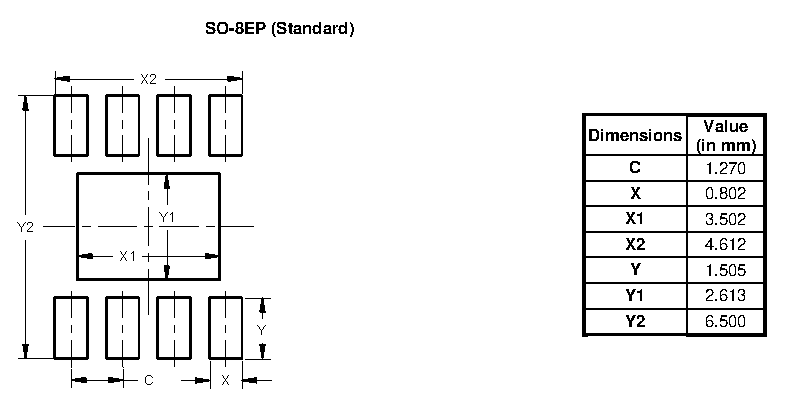
\includegraphics[width=0.7\textwidth]{Chapters/Figures/chapter5/footprint_AP64501.pdf}
	\caption{Recommended solder pad pitch and dimensions for the AP64501 synchronous buck converter~\cite{AP64501}.}
	\label{fig:footprint_AP64501}
\end{figure}

For the ICs and modules whose footprints are not provided by default by the software, internet research was conducted in order to find them -- \url{https://www.snapeda.com/} and \url{https://pt.mouser.com/} were the two websites accessed for such purpose, since these are known to provide trustworthy footprints.

Regarding resistors, unless otherwise stated, all should have a 0805 \gls{SMD} package footprint and a tolerance of 5\%. The standard 0805 package size measures $0.08 \times 0.05$ inches (length $\times$ width), which corresponds, in the metric system, to a 2012 package size, at $2.0 \times 1.25$ millimetres (length $\times$ width).
Capacitors should also have a 0805 SMD package footprint and be rated for 50V, unless otherwise stated.
As for the remaining components, i.e. MOSFETs, diodes, inductors, ferrites, crystal and connectors, their footprint depends on the application.
Datasheets of ICs and modules usually refer the characteristics and/or models to use in a typical implementation.

To effectively design the board's layout, KiCad provides a PCB editor that places the assigned footprints in single editing window. This premature placement must then be rearranged according to the respective component's location in the circuit, in the most efficient way possible among other partner components. The PCB editor also displays white lines (known as ``ratsnest lines'') that connect the different components' pads to each other, just as defined in the schematic design. This subsequently helps in the routing process (i.e. effectively connecting every component with tracks (also known as ``traces''), vias and zones). Figure~\ref{fig:ratsnest} shows an early version of the layout for the external power supply region of the system, which is connected to the LTC4012 and to the external power voltage reference (top left area of the schematic of Figure~\ref{fig:LTC4012_circuit}).

\begin{figure}[h]
	\centering
	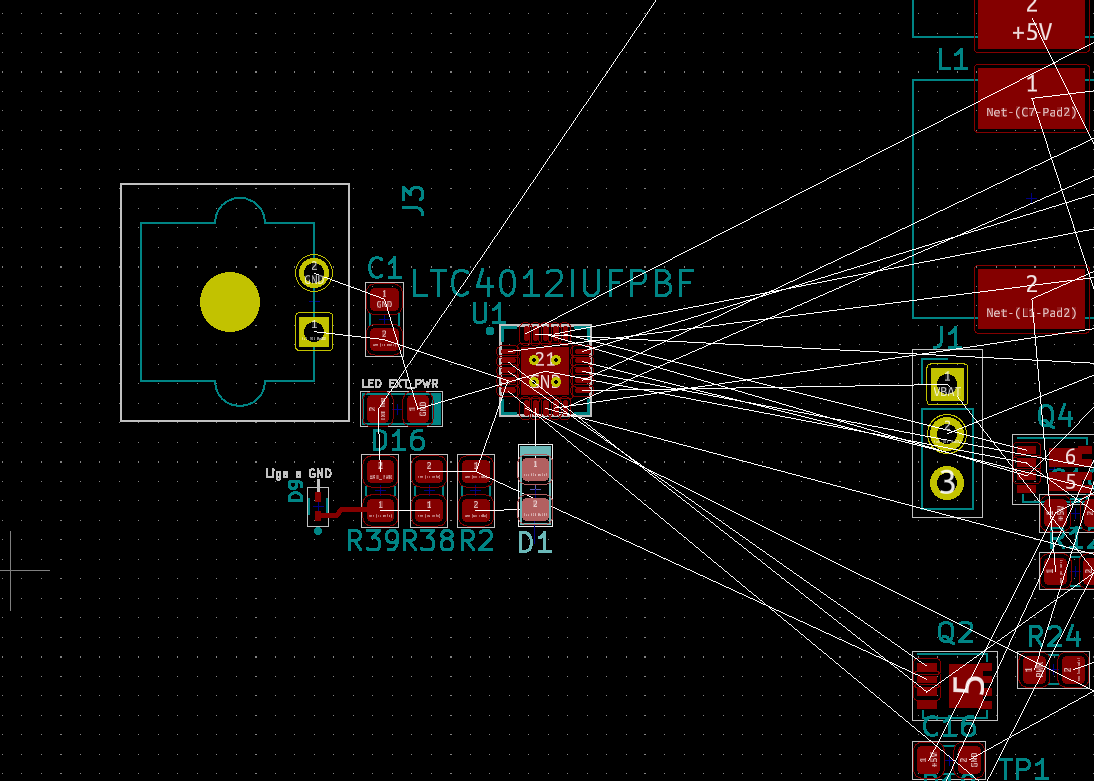
\includegraphics[width=0.8\textwidth]{Chapters/Figures/chapter5/ratsnest.png}
	\caption{Unconnected footprints for the external power supply region of the system (early version).}
	\label{fig:ratsnest}
\end{figure}


%s--Ss--Ss--Ss--Ss--Ss--Ss--Ss--Ss--Ss--Ss--Ss--Ss--Ss--Ss--Ss--Ss--Ss--Ss--S
\subsubsection{Control Unit and USB 2.0 Hub}\label{sec:5111_CM4_LAN9514}

%0. falar do placement estar concluido:
To arrange all components in the best way possible, one has to take into account a provisional routing, to achieve a good placement in the least amount of iterations possible. For that, it's considered good practice to start by imagining and experimenting with placing and routing of the high-speed zones of the circuit first. For this project, that would concern the CM4's high-speed side and the LAN9514's USB side. Figure~\ref{fig:placement_CM4_LAN9514} focuses on the final component placement of the CM4 module and the LAN9514 hub on the board.

\begin{figure}[h]
	\centering
	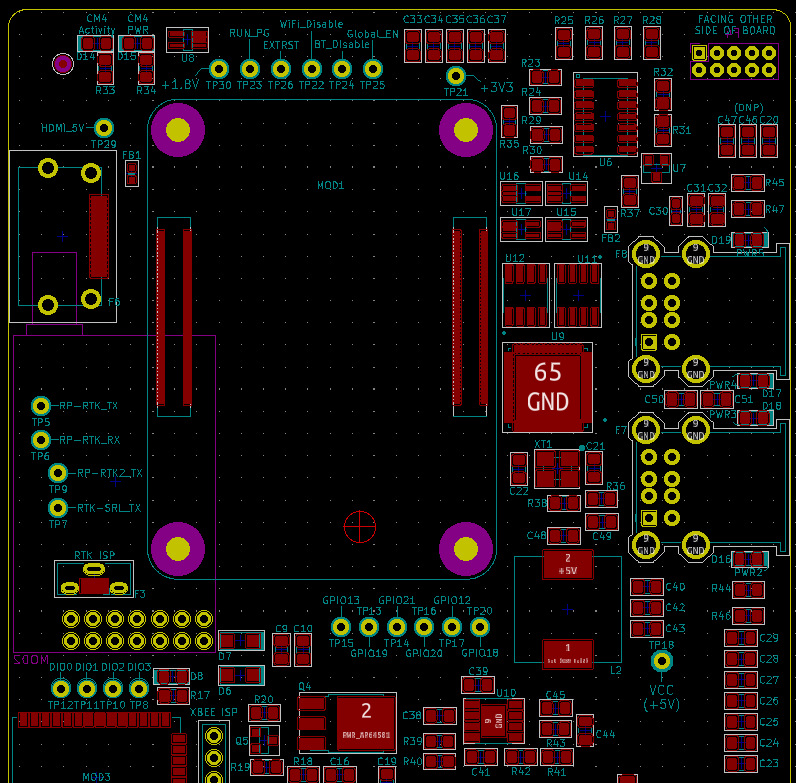
\includegraphics[width=0.7\textwidth]{Chapters/Figures/chapter5/placement_CM4_LAN9514.png}
	\caption{Final placement of the CM4 and LAN9514 circuits' components.}
	\label{fig:placement_CM4_LAN9514}
\end{figure}%placement_CM4_LAN9514

The location of the peripheral ports (HDMI and USB) must also be accounted for. It is common for these to be placed near the limits of the board so that user access is facilitated.

After placing the downstream USB connectors near the right edge of the board, the LAN9514 hub was placed to the left of these, in way that it would be more-or-less equidistant from each to account for the routing of the high-speed USB data traces. After defining a position for the hub, its most important component was placed: the crystal oscillator XT1. This part must be the closest possible to its respective hub's pins, in order to settle a trustworthy clock frequency from which the IC will rely on. Followed by the crystal's capacitors, the remaining components were placed the nearest possible to the hub.

Setting the CM4 immediately to the left of the USB hub, choosing to locate the HDMI port on the left edge of the board, near the CM4's HDMI pins, was straightforward.

The power and activity LEDs (D15 and D14, respectively) were placed near the top left edge of the board (i.e. top left of Figure~\ref{fig:placement_CM4_LAN9514}), a simple and easy-to-remind location, specially for the testing phase.

All the CM4's test points (e.g. +3V3, WL\_nDisable, GPIOx, etc.) are located either near the top or bottom of the module (MOD1) -- also easy-to-remind and to reach locations.

Regarding the LAN9514's bypass capacitors, these were placed near the top-middle of the board, as well as above and below the downstream USB connectors (also visible in Figure~\ref{fig:placement_CM4_LAN9514}).


%s--Ss--Ss--Ss--Ss--Ss--Ss--Ss--Ss--Ss--Ss--Ss--Ss--Ss--Ss--Ss--Ss--Ss--Ss--S
\subsubsection{Power Selector}\label{sec:5112_LAN9514}

The next step taken was the placement of the power selector circuit. In the applications information sections of the LTC4012 datahseet (\cite{LTC4012}), a list of PCB layout considerations are provided. Regarding these, it is recommended to follow a specific priority order, as to ensure a proper layout. The notes go through the best possible layout for the switch node of the battery charger and its importance in the design. This switch node corresponds to the point where diode D4 and inductor L1 meet (see Figure~\ref{fig:LTC4012_circuit}). The suggested priority list for the LTC4012 layout starts with notes on the correct placement of the switching FETs (Q2 and Q9) relative to the IC and its input capacitors, running through the inductor, current sense resistors, output capacitors and notes regarding PCB layer, trace and via topology. Following these guidelines resulted in the component placement represented on the right side of Figure~\ref{fig:placement_Power_Selector_and_BQ29209}, where the switching FETs, input capacitors and inductor are clearly visible close and around the LTC4012 footprint.

\begin{figure}[h]
	\centering
	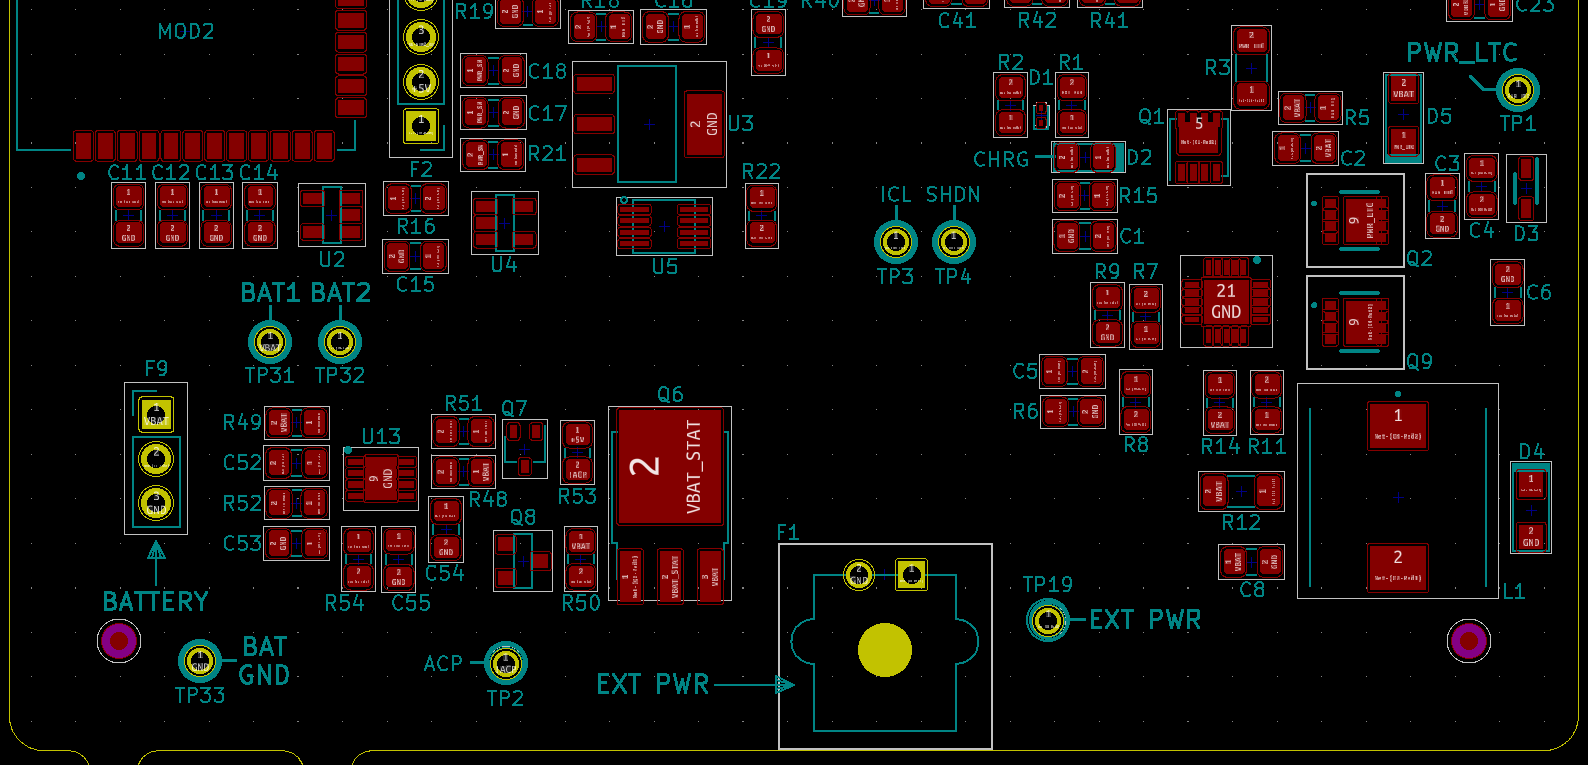
\includegraphics[width=0.7\textwidth]{Chapters/Figures/chapter5/placement_Power_Selector_and_BQ29209.png}
	\caption{Final placement of the Power Selector and Battery Balancer circuits' components.}
	\label{fig:placement_Power_Selector_and_BQ29209}
\end{figure}%placement_Power_Selector_and_BQ29209


%s--Ss--Ss--Ss--Ss--Ss--Ss--Ss--Ss--Ss--Ss--Ss--Ss--Ss--Ss--Ss--Ss--Ss--Ss--S
\subsubsection{Battery Balancer}\label{sec:5113_BQ29209}

This IC's datasheet (\cite{bq29209}) also provides a dedicated section highlighting recommended layout suggestions for users. Among other notes, these encourage the designer to place the input capacitors as close as possible to the IC in order to filter out the most amount of noise possible. This resulted in the placement shown on the lower left zone of Figure~\ref{fig:placement_Power_Selector_and_BQ29209}.


%s--Ss--Ss--Ss--Ss--Ss--Ss--Ss--Ss--Ss--Ss--Ss--Ss--Ss--Ss--Ss--Ss--Ss--Ss--S
\subsubsection{Voltage Converter}\label{sec:5114_VoltageConverter}

Similar to the previous IC's datasheets,~\cite{AP64501} singles important guidelines for a thorough layout of the AP64501's circuit. These guidelines are laid out in list form, starting by addressing the recommended copper thickness for the carrier board for the IC (due to the maximum 5A output current), followed by the importance of the placement of the input capacitors and inductor (L2) as close as possible to their respective terminals on the converter. More specifically, the input capacitors should be placed close to the power supply (VIN) of the IC, and the inductor close to the switching terminal (SW) -- similar to the layout topology addressed by the LAN9514's datasheet. After this, the list focuses on output capacitors, feedback components, and finally PCB layers and vias. A layout schematic example is also provided, and is represented in Figure~\ref{fig:AP64501_layout_Datasheet}.

% meter aqui AP64501 layout - datasheet
\begin{figure}[h]
	\centering
	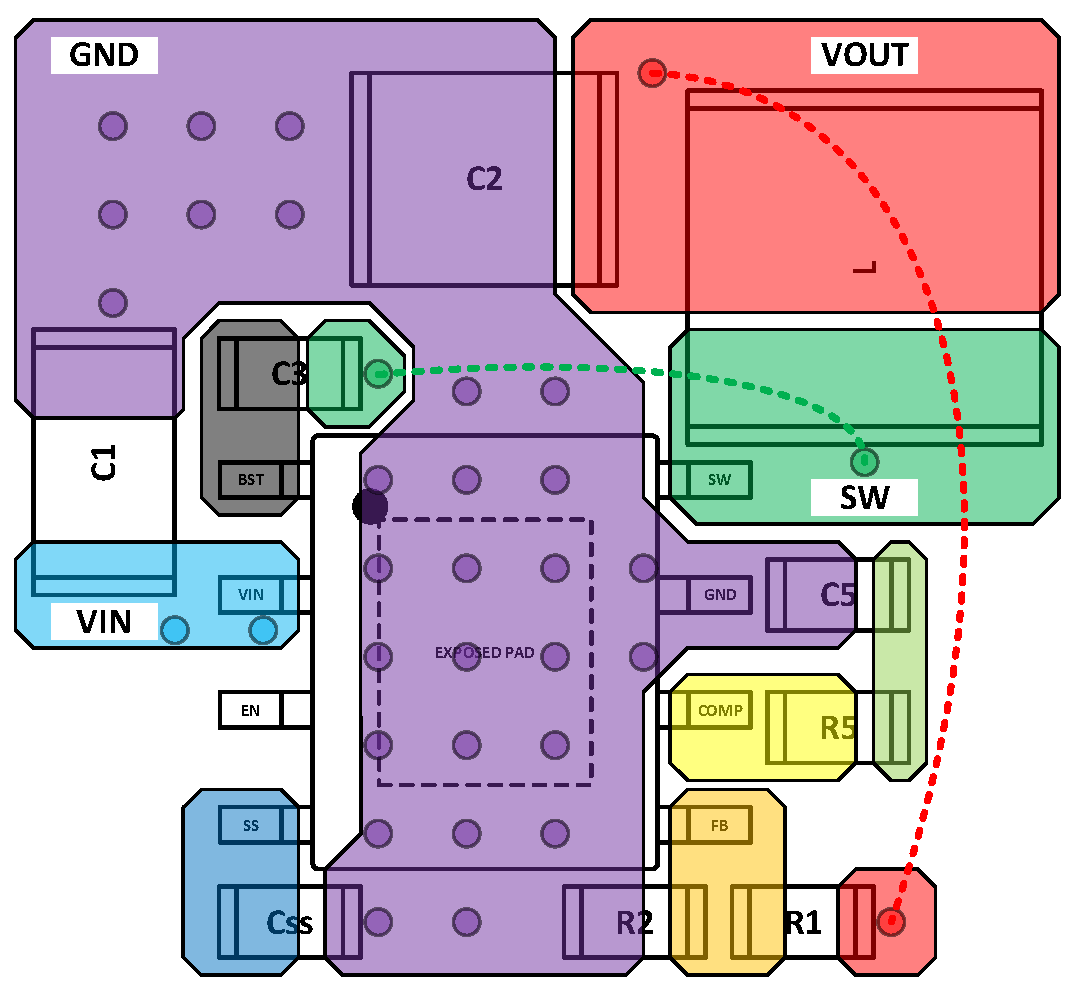
\includegraphics[width=0.5\textwidth]{Chapters/Figures/chapter5/AP64501_layout_Datasheet.pdf}
	\caption{Recommended layout for the AP64501 synchronous buck converter's circuit~\cite{AP64501}.}
	\label{fig:AP64501_layout_Datasheet}
\end{figure}

Taking all these notes into account resulted in the component placement depicted on Figure~\ref{fig:placement_VoltageConverter}.

\begin{figure}[h]
	\centering
	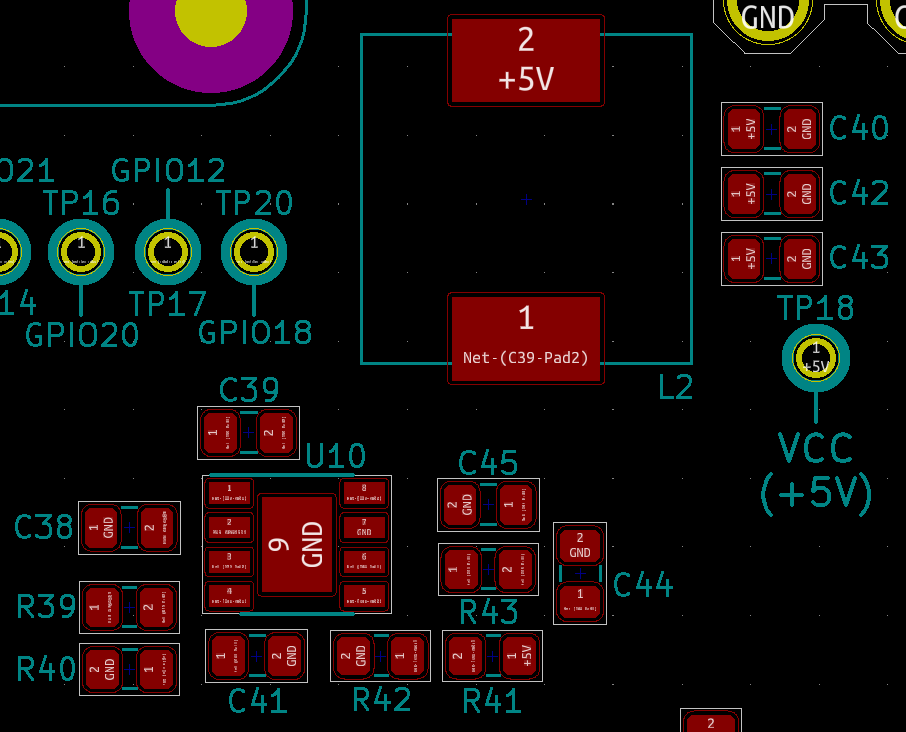
\includegraphics[width=0.6\textwidth]{Chapters/Figures/chapter5/placement_VoltageConverter.png}
	\caption{Final placement of the Voltage Converter circuit's components.}
	\label{fig:placement_VoltageConverter}
\end{figure}%placement_VoltageConverter


%s--Ss--Ss--Ss--Ss--Ss--Ss--Ss--Ss--Ss--Ss--Ss--Ss--Ss--Ss--Ss--Ss--Ss--Ss--S
\subsubsection{Power Switch}\label{sec:5115_PowerSwitch}

The power switch circuit placement revealed itself to be very simple, only with notes from~\cite{SN74LVC2G74DCTR} to pay attention to upon the routing phase -- addressed in Section~\ref{sec:52_Routing}. Figure~\ref{fig:placement_PowerSwitch} shows the arrangement made for this circuit, which basically surrounds the main ICs (the D-type flip-flop, the inverter, and the voltage regulator) with their function-defining components.

\begin{figure}[h]
	\centering
	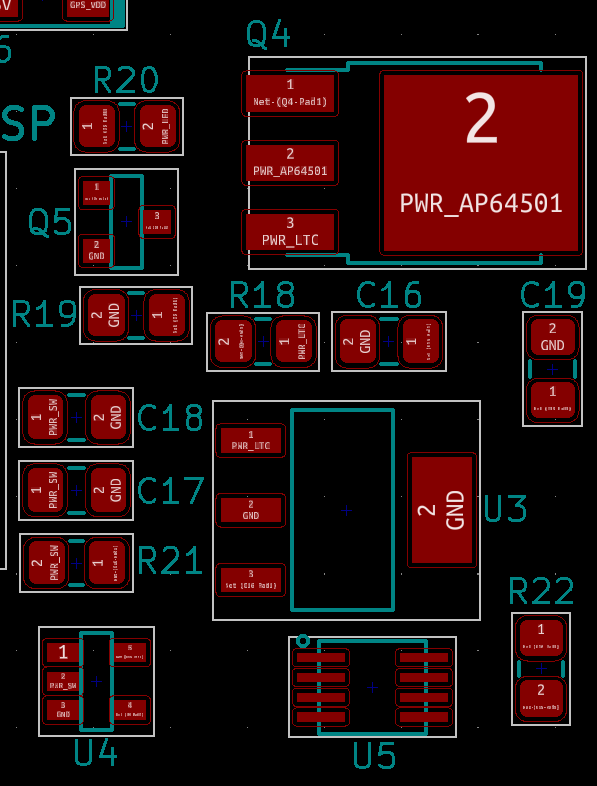
\includegraphics[width=0.4\textwidth]{Chapters/Figures/chapter5/placement_PowerSwitch.png}
	\caption{Final placement of the Power Switch circuit's components.}
	\label{fig:placement_PowerSwitch}
\end{figure}%placement_PowerSwitch


%s--Ss--Ss--Ss--Ss--Ss--Ss--Ss--Ss--Ss--Ss--Ss--Ss--Ss--Ss--Ss--Ss--Ss--Ss--S
\subsubsection{Human-Machine Interface}\label{sec:5116_HMI}

Figure~\ref{fig:placement_HMI} shows the placement of the LM2901 comparator's circuit (previously represented on the left of Figure~\ref{fig:HMI_circuit}).
Placement for this part of the system also proved to be straightforward, due to the reduced number of components (mainly resistors), which were simply laid out around comparator U6.

As explained previously, the status voltage from the comparator flows to the HMI itself through the connection of two 2.54mm pitch pin headers, F4 and F5. F4 is placed close to U6, as well as to the top right corner of the board, on its opposite side (see Figure~\ref{fig:placement_HMI}, left). It is supposed to be connected to F5 to power all indication LEDs and push-button SW1, as well as to establish nets PWR\_SWITCH, PWR\_LED and EXT\_PWR. The right side of Figure~\ref{fig:placement_HMI} shows a small separate PCB just for the HMI. The reason for this separate board is due to its specific user-accessible location on the outside of the base station's casing.

\begin{figure}[h]
	\centering
	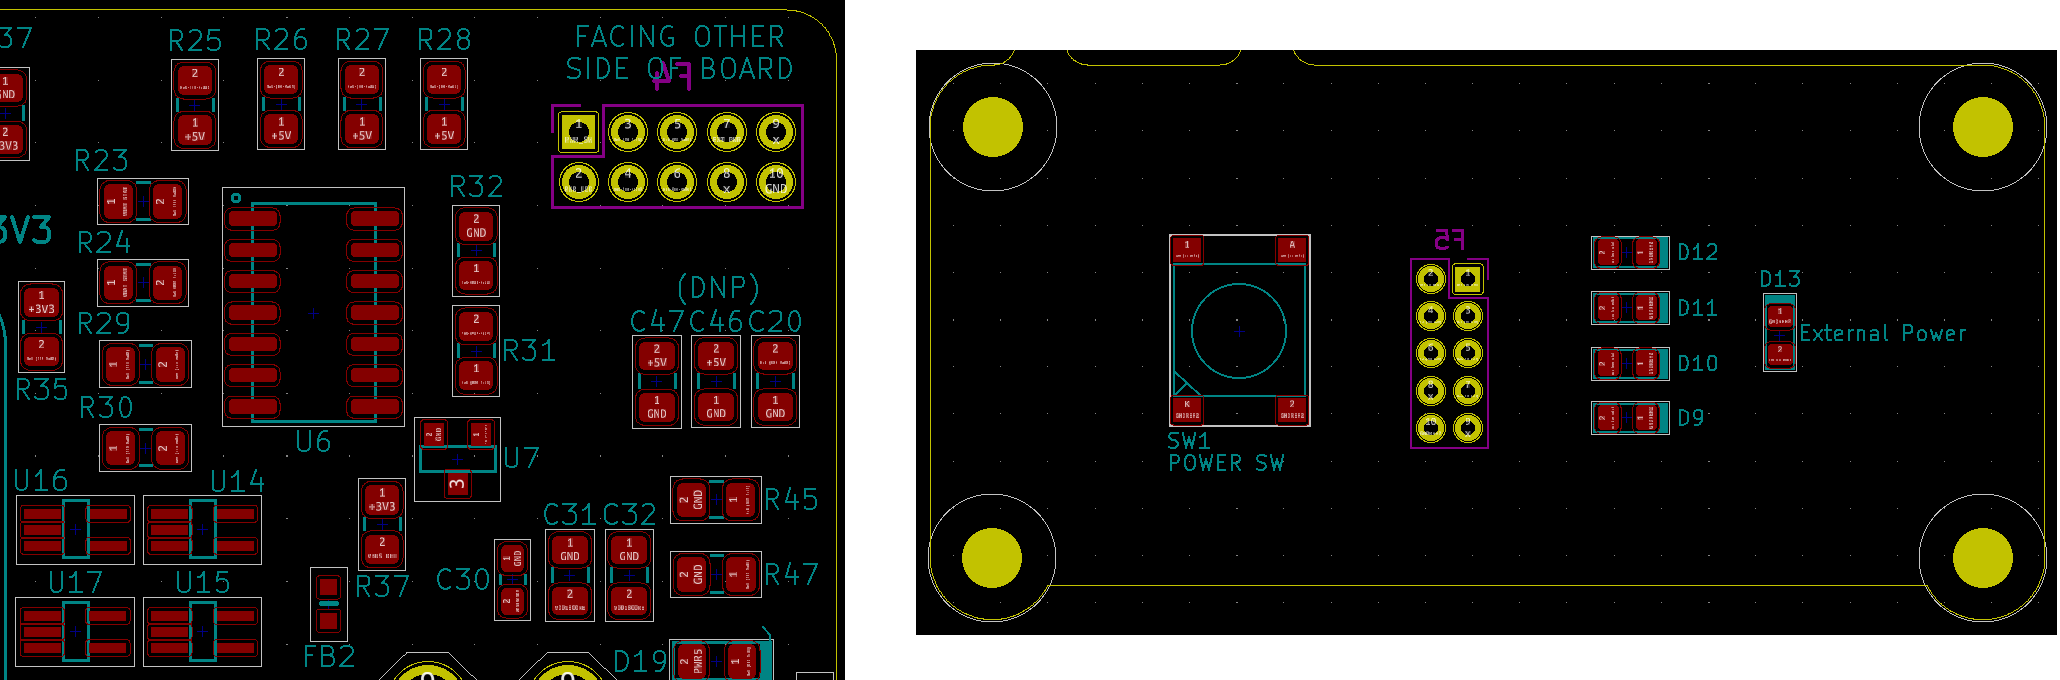
\includegraphics[width=0.7\textwidth]{Chapters/Figures/chapter5/placement_HMI.png}
	\caption{Final placement of the status voltage comparator (left) and HMI (right) circuits' components.}
	\label{fig:placement_HMI}
\end{figure}%placement_HMI


%s--Ss--Ss--Ss--Ss--Ss--Ss--Ss--Ss--Ss--Ss--Ss--Ss--Ss--Ss--Ss--Ss--Ss--Ss--S
\subsubsection{GNSS module and Wi-Fi Transceiver}\label{sec:5117_ZED_XBEE}

Aside from connector F4, the GNSS module was the only system part to be placed on the back side of the main board, since this was the most convenient location due to its mechanical structure (i.e. because the module itself consists on a small PCB with a pin header soldered on it). The remaining components connected to the GNSS module's circuit, namely the RTK ISP connector, input capacitors C9 and C10, and diodes D6 and D7 are placed on the front side of the main board, near the opposite location of the module itself, along with the RTK data test points. All this can be seen on the top portion of the left side of Figure~\ref{fig:placement_ZED_XBEE}.

\begin{figure}[h]
	\centering
	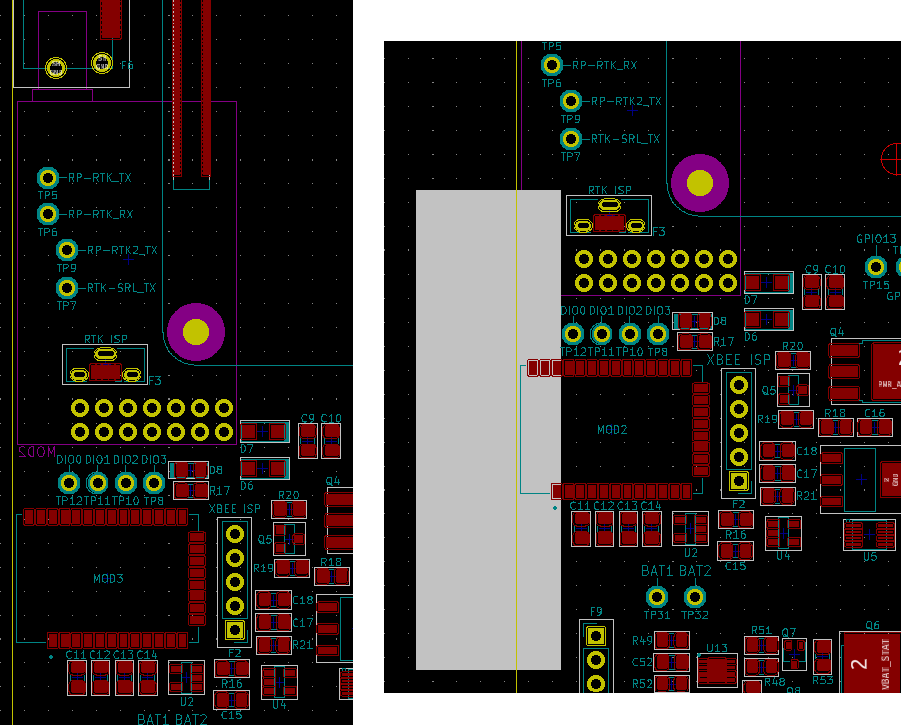
\includegraphics[width=0.6\textwidth]{Chapters/Figures/chapter5/placement_ZED_XBEE.png}
	\caption{Final placement of the GNSS module and Wi-Fi Transceiver circuits' components (left); Antenna keepout area for the XBee 3 RF module (right).}
	\label{fig:placement_ZED_XBEE}
\end{figure}%placement_ZED_XBEE

As for the Wi-Fi transceiver, i.e. the XBee 3 RF module,~\cite{XBee} provides layout design notes to help achieve the best antenna performance possible. Since the XBee module used in this project is known as the its ``micro chip'' version, the notes for this version are the ones to pay attention to. These state that non-metal enclosures are preferred, and that all metal parts of the system -- either internal or external in respect to the main board -- must be kept at the maximum distance possible from the module's antenna. For that,~\cite{XBee} also provides a graphic visualization of a recommended antenna keepout area to implement. The righ side of Figure~\ref{fig:placement_ZED_XBEE} shows such area.

After assessing these guidelines, the placement of this circuit's components was standard when compared to the previous sections, with output capacitors C11-C14 of the U2 LDO placed as close as possible to its output, as well as to the VCC input (pin 2) of the XBee module. All test points for the latter (DIO0-DIO3) are placed above it.

%   dizer que é importante o cristal estar mais perto possivel do LAN, porque o routing desta parte do circuito é critica;
%   importante as USB downstream ports estarem o mais perto possivel do LAN
%   ver se me lembro de mais regras...
%   definiu-se um limite experimental para a placa ($100 \times 70$ mm (length $\times$ width)) e acabou por se aumentar para $129 \times 90$ mm (length $\times$ width).

Concluding the placement of every sub-circuit, the remaining placement-related task is to assign these to a roughly specific location on the board. Choosing the board's dimensions settles the placement phase. For the main board, the final size was set to $129 \times 90$ mm (length $\times$ width). As for the HMI board, the same $30 \times 60$ mm (length $\times$ width) measurements from the previous beRTK\textsuperscript{\textregistered} version were kept unaltered. Figure~\ref{fig:placement_FULL} shows the final placement of the entire system within the board's defined limits.

\begin{figure}[h]
	\centering
	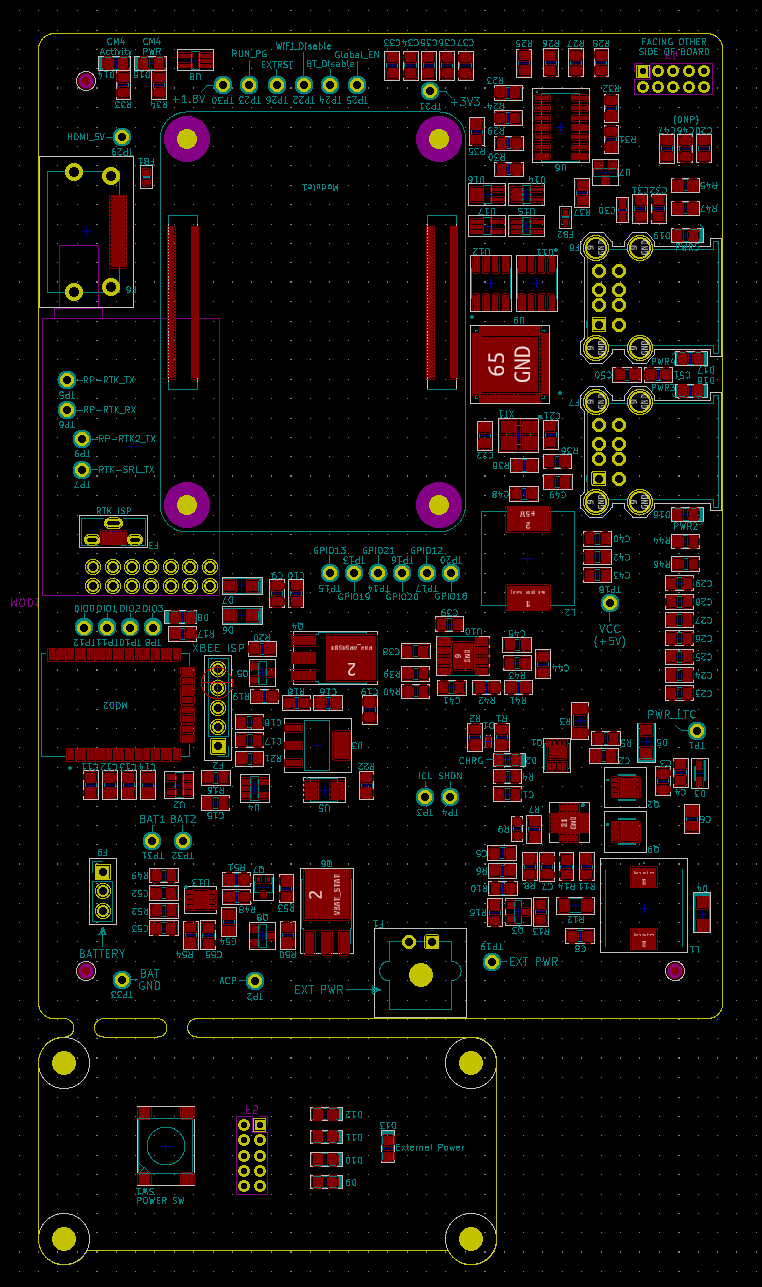
\includegraphics[width=0.6\textwidth]{Chapters/Figures/chapter5/placement_FULL.png}
	\caption{Final placement of the new beRTK\textsuperscript{\textregistered} system within the board's defined limits.}
	\label{fig:placement_FULL}
\end{figure}%placement_FULL

\subsection{Routing}\label{sec:52_Routing}

%   depois começa o routing:
After placement, routing is the process that connects every component to each other, and at the PCB level, this can either occur with traces, vias or copper pours.

%1. falar das minimum design rules da eurocircuits:
Right before beginning the routing process, the board setup must be done in the KiCad PCB editor. This critical step consists in defining the board's stackup (i.e. number of layers, copper pour thickness) and design rules. Depending on the chosen PCB manufacturer, these definitions may vary. For this project, the selected board manufacturer was Eurocircuits, a ``specialist manufacturer and assembler of prototype and small series PCBs''\footnote[19]{Available at \url{https://www.eurocircuits.com/who-are-we/}.}. For KiCad users, Eurocircuits provides sets of minimum design rules (i.e. design constraints) for various PCB stackup types that may vary in either single or double-sided designs, number of layers, or copper thickness. The following set of constraints presented are for a four-layer board with a base copper thickness of $18 \mu$m and $35 \mu$m, for the outer (OL) and inner (IL) layers, respectively\footnote[20]{Eurocircuit's KiCad design rules for other board stackups are available at \url{https://www.eurocircuits.com/blog/kicad-design-rules/}.}:
\begin{itemize}
	\item Min. trace width, OL: 0.150mm;
	
	\item Min. clearance, OL: 0.150mm;
	
	\item Min. trace width, IL: 0.150mm;
	
	\item Min. clearance, IL: 0.150mm;

	\item Min. via drill diameter (tool size): 0.35mm;
	
	\item Min. via pad diameter, OL: 0.600mm;
	
	\item Min. via pad diameter, IL: 0.600mm.
\end{itemize}
Therefore, the board's stackup defined by these constraints was selected as the stackup for the new beRTK\textsuperscript{\textregistered}'s board. The four-layer order chosen (from the top-down) was signal-power-power-signal (in this case: F.Cu-GND-PWR-B.Cu; F.Cu and B.Cu refer to the board's front and back copper signal layers).

A second Eurocircuits' tool can be used to obtain the board's physical stackup dimensions -- the ``Buildup Editor''. This tool allows the user to select the board's desired number of layers, along with its thickness and base material (among other specifications), and provides a preview of its layers' stackup with the expected physical dimensions in millimetres. Figure~\ref{fig:buildup_4layer} shows the Eurocircuits Buildup Editor's calculation of the physical stackup for a four-layer, 1.55mm thick PCB with an FR-4 Improved base material.

\begin{figure}[h]
	\centering
	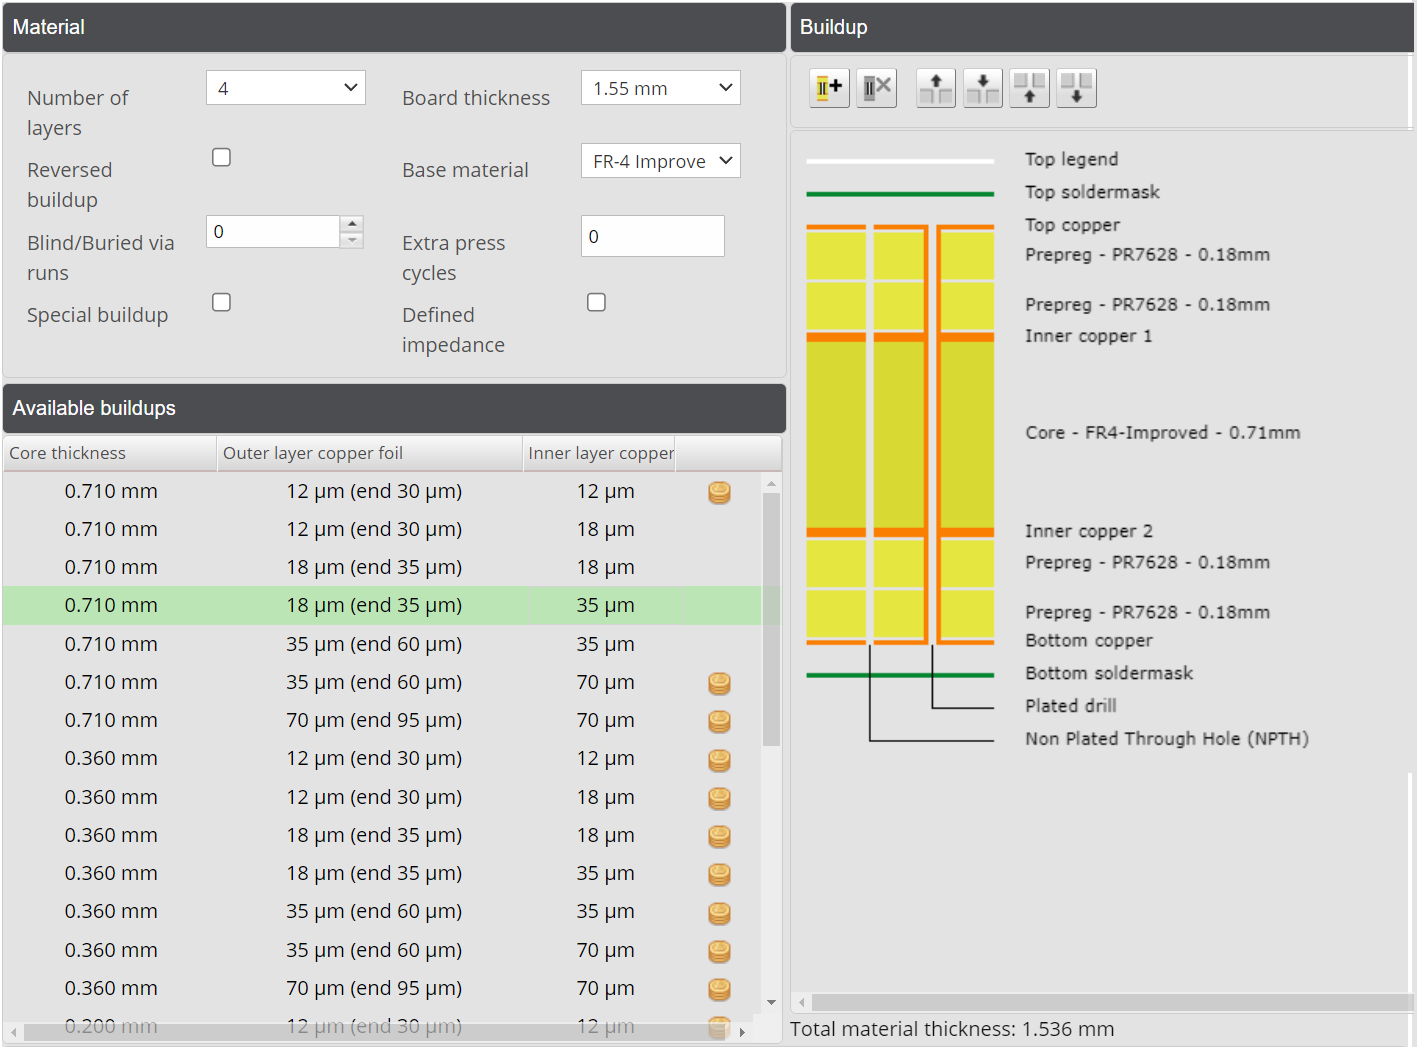
\includegraphics[width=0.8\textwidth]{Chapters/Figures/chapter5/buildup_4layer.png}
	\caption{Eurocircuits Buildup Editor's calculation of the physical stackup of a four-layer, 1.55mm thick PCB with an FR-4 Improved base material (available in the Eurocircuits website).}
	\label{fig:buildup_4layer}
\end{figure}

\noindent The values displayed in the diagram of Figure~\ref{fig:buildup_4layer} can thus be applied to the physical stackup tab of KiCad's board setup manager, as shown in Figure~\ref{fig:KiCad_buildup_4layer}.

\begin{figure}[h]
	\centering
	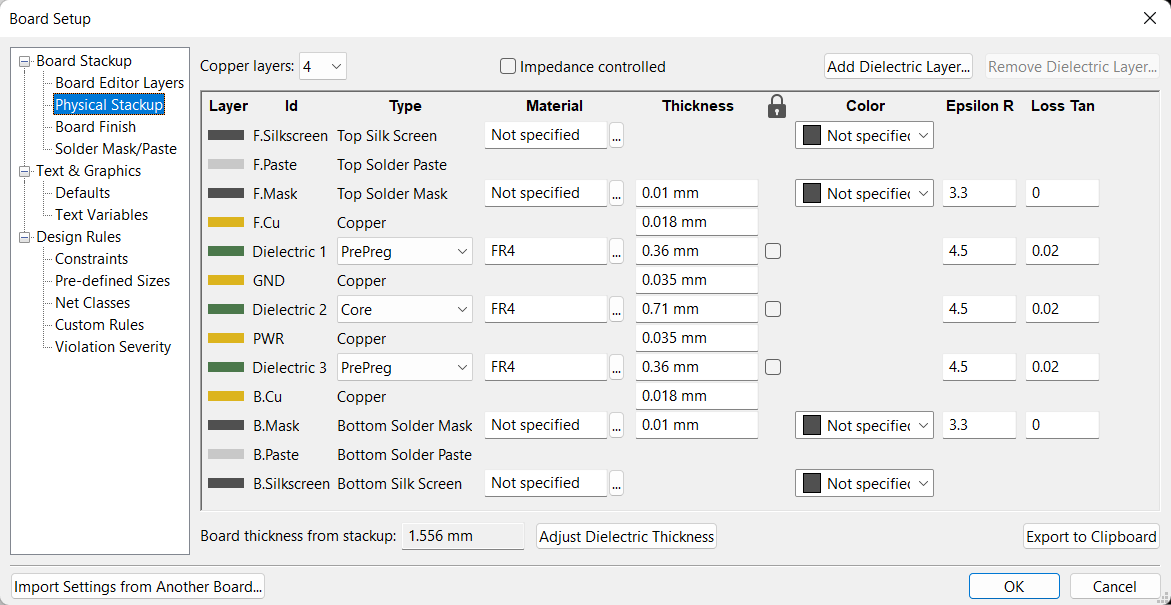
\includegraphics[width=0.8\textwidth]{Chapters/Figures/chapter5/KiCad_buildup_4layer.png}
	\caption{Board's physical stackup dimensions applied in KiCad's board setup manager.}
	\label{fig:KiCad_buildup_4layer}
\end{figure}

After setting up the physical stackup of the board and defining its design rules' constraints, the net classes must be defined. For specified nets (e.g. VBAT, PWR\_LED, GPS\_VDD, etc.), these dictate the actual PCB trace's width and clearance, as well as the size of vias to use. To define a net's trace dimensions, key parameters such as its current flow capacity (in A) temperature rise above ambient ($\Delta T$, in $\degree$C), and copper resistivity ($1.72 \cdot 10^{-8} \Omega$m) must be taken into account. KiCad also provides a PCB calculator tool for trace width calculation, shown in Figure~\ref{fig:PCB_calculator}.

\begin{figure}[h]
	\centering
	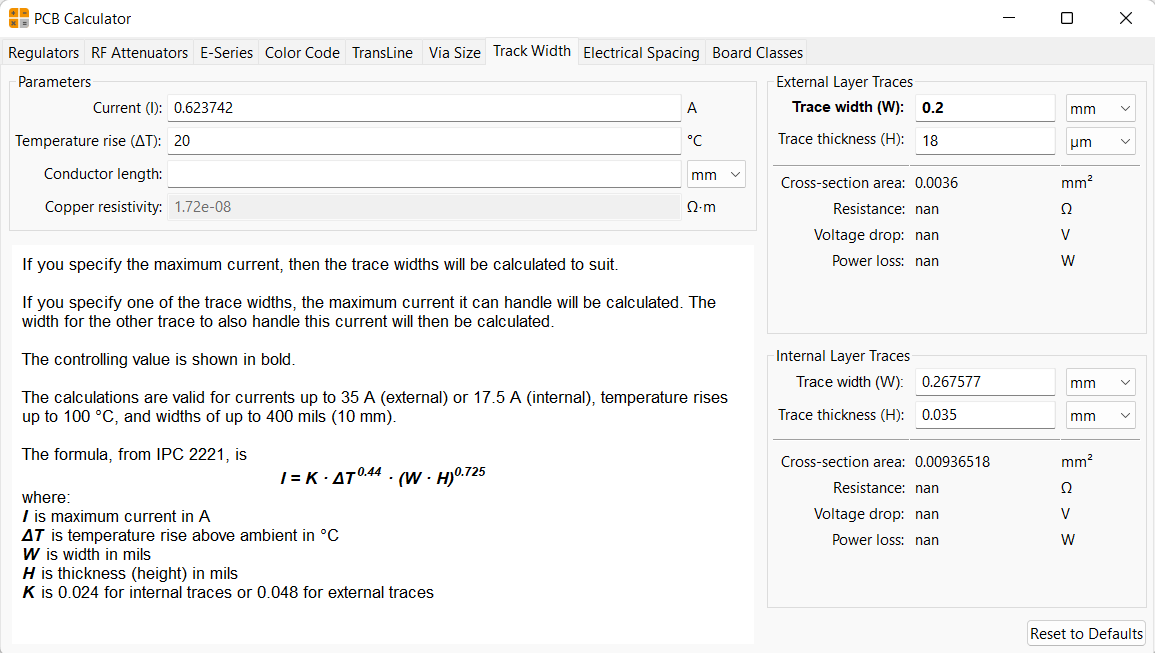
\includegraphics[width=0.8\textwidth]{Chapters/Figures/chapter5/PCB_calculator.png}
	\caption{KiCad's PCB track width calculator used.}
	\label{fig:PCB_calculator}
\end{figure}

Looking at Figure~\ref{fig:PCB_calculator}, it is possible to see that the calculator accepts either parameter or layer trace dimension inputs. As stated in the figure, the IPC 2221 (the Generic Standard on Printed Board Design) formula to calculate the trace's maximum current allowed is given by (\ref{eq:I_trace}):

\begin{equation}\label{eq:I_trace}
	I = K \cdot \Delta T^{0.44} \cdot (W \cdot H)^{0.725}\,\medskip
\end{equation}
\noindent Where:
\begin{itemize}
	\item $I$ -- Maximum current that will flow through the trace, in A;
	
	\item $\Delta T$ -- Temperature rise above ambient, in $\degree$C;
	
	\item $W$ -- Trace width, in mils (1 mils $=$ 0.0254 millimeters);
	
	\item $H$ -- Trace thickness (i.e. height), in mils;
	
	\item $K$ -- 0.024 for internal traces or 0.048 for external traces.
\end{itemize}

For this project, four net classes were defined for the routing process:

\begin{itemize}
	\item Default net class -- Corresponds to every net in the circuit that is not HDMI, USB, or power-related. Examples for such are the nets that connect each of the four outputs of comparator U6 to pin header F4, for the status voltage (Figure~\ref{fig:HMI_circuit});
	
	\item Power net class -- Corresponds to every net in the circuit where considerable amount of current is expected to flow. Examples for such are the PWR\_SUPPLY and 5V nets;
	
	\item USB net class -- Corresponds to every USB-related net in the circuit;
	
	\item HDMI net class -- Corresponds to every HDMI-related net in the circuit.
\end{itemize}

It must be noted that, for this project, routing is only be done on the outer (i.e. signal) layers of the board. The inner layers are defined in zones. The GND layer is a single, continuous layer that serves as a ground reference for every component, IC, and module; the PWR layer is separated into different zones, to account for dissipation of the circuit's power needs, i.e. to avoid concentrating large amounts of power solely on the outer layers' traces.

Starting by defining the ``Default'' net class: choosing a trace width of 0.20mm, a trace thickness of $18 \mu$m (as defined earlier in the board stackup manager), and a common $\Delta T$ temperature rise of $20 \degree$C, plugging those values into KiCad's PCB calculator, a maximum current of approximately 0.624A is allowed to flow through the trace (see Figure~\ref{fig:PCB_calculator}) before any type of trace overheat or breakdown occurs. Requirement \textbf{RTKBS.MAIN.PWS.040} states that the base station ``shall not exceed an average of 400mA of current consumption at 5VDC voltage level''. If every ``Default'' net at 5V consumes the 400mA maximum stipulated, the 0.20mm trace thickness for these nets will be large enough, since it can withstand up to 624mA of current. For this net class, vias were kept at the minimum size allowed by design rule constraints.

The ``Power'' net class encompasses the routing for power-hungry devices in the system, and therefore it must account for larger amounts of current that may flow. Even though the entire system is expected to consume a low amount of power, the Power net class traces and vias should be larger when compared to the Default net class, in case large surges of current or unexpected temperature rises occur. A trace width of 0.50mm was chosen, which allows a maximum current flow of approximately 1.212A. Vias for this net class were defined at a total diameter of 0.80mm with a finished hole size of 0.40mm.

Defining the correct trace dimensions for high-speed circuits is more critical than for default nets or even power nets, for that matter. This is because high-speed circuits are subject to problems such as signal reflection, coupling and crosstalk, if designed poorly. The intrinsic inductive and resistive nature of traces is often overlooked for typical low-speed circuitry. The same occurs for the capacitive effect between traces, which calls back to the ``clearance between traces'' parameter. However, for high-speed circuits, these characteristics must never be dismissed, and defining this type of traces is called ``impedance matching''.

Referring to Section 7.1.1.3 of the USB 2.0 Specification, it defines that the board traces for the USB 2.0 data differential pair must bear a nominal differential characteristic impedance of $90 \Omega \pm 15\%$, which means that this impedance value may range from $[76.5,\, 103.5]\Omega$. The first step in calculating the differential impedance ($Z_{DIFF}$) of a USB 2.0 differential pair of traces is to know the single-ended impedance ($Z_0$) value, which can be calculated through expression (\ref{eq:USB_impedance_Z_0}):

\begin{equation}\label{eq:USB_impedance_Z_0}
	Z_0 = \frac{87}{\sqrt{\epsilon_r + 1.41}} \cdot \ln \left(\frac{5.98 \cdot h}{0.8 \cdot w + t}\right)\,\medskip
\end{equation}
$\epsilon_r$ is the substrate's relative permittivity (i.e. dielectric constant) and, for the FR-4 material, is typically equal to 4.5.
Figure~\ref{fig:USB_differential_pair} shows the cross-section of a PCB with a differential pair of traces. The traces' and board's dimensions highlighted by the variables are some of the parameters used for the calculation of $Z_0$ and are known as:
\begin{itemize}
	\item $w$ -- Trace width, in meters;
	
	\item $d$ -- Trace spacing, in meters;
	
	\item $t$ -- Trace thickness, in meters;
	
	\item $h$ -- Dielectric thickness, in meters.
\end{itemize}

% meter aqui traces e board diagram
\begin{figure}[h]
    \centering
    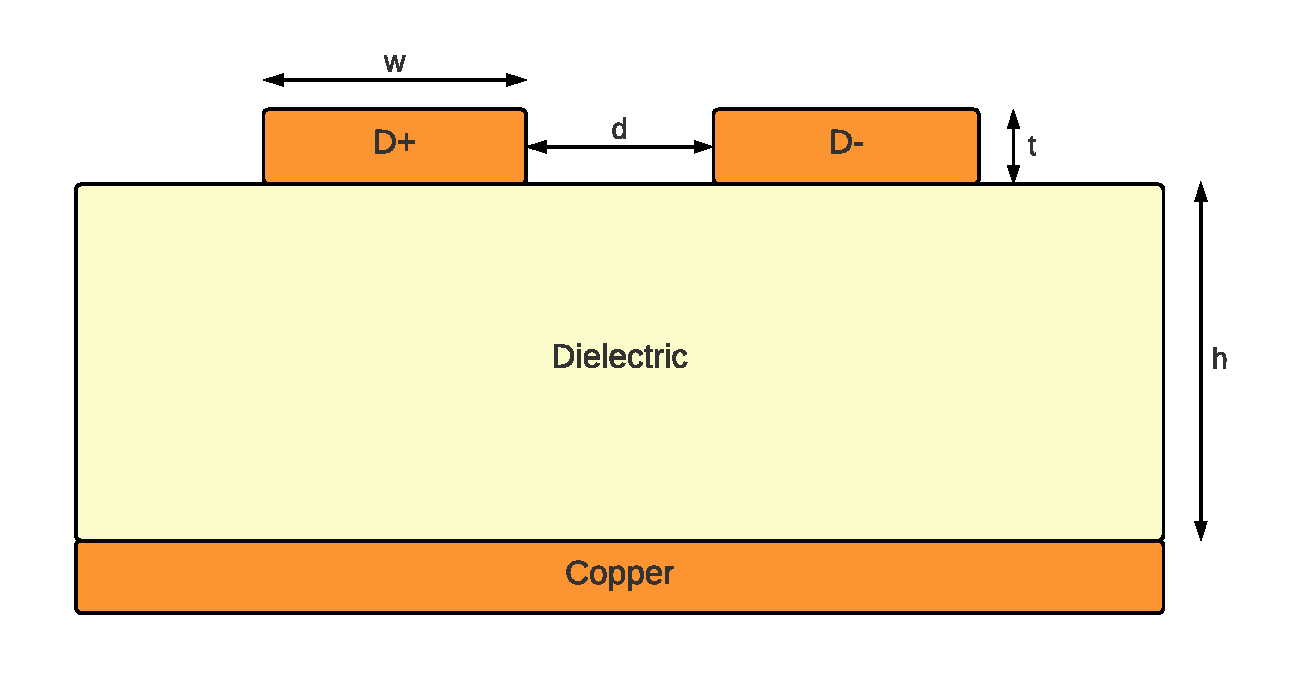
\includegraphics[width=0.5\textwidth]{Chapters/Figures/chapter5/USB_differential_pair.pdf}
    \caption{Cross-section of a PCB with a differential pair of traces.}
    \label{fig:USB_differential_pair}
\end{figure}

%parei aqui. agarrar na calculadora e fazer a conta para Z_0.

Expression (\ref{eq:USB_impedance_Z_DIFF}) allows calculating the differential impedance ($Z_{DIFF}$) of a USB 2.0 differential pair of traces. For that : 

\begin{equation}\label{eq:USB_impedance_Z_DIFF}
	Z_{DIFF} = 2 \cdot Z_0 \cdot \left(1 - 0.48 \cdot e^{-0.96 \cdot \frac{d}{h}}\right)\,\medskip
\end{equation}



%2. falar das minimum design rules que eu usei, que sao um pouco diferentes
%3. dizer a thickness da placa, 4 layers -- 2 signal, 2 pwr -- mostrar a janela do kicad
%4. falar das thickness das tracks de power, de signal, tamanho das vias de power, de signal. clearance
%4.1 definiram se os signal, power, GND planes.
%5. dizer que o primeiro routing que se fez foi o mais critico --  USB e HDMI -- que tambem têm tracks com tamanhos especificos -- falar e mostrar as contas desses tamanhos (impedance matching).
%4. importante que as power tracks passem pelos capacitors primeiro e so depois vao para o power plane (5V), para que os condensadores possam cumprir devidamente o seu propósito de bypassing.



-- $20 \mu$F ceramic capacitors were chosen for both the power inputs and power output of the LTC4012. 

-- As mentioned before, the top and bottom power FETs Q2 and Q9, along with inductor L1 are vital to the PWM control architecture. These components are part of the sub-circuit that starts from the +15VDC source of power and passes across FET Q1 (connected to pin INFET), sense resistor R3, 
This sub-circuit forms the ``power supply rail'', and upon layout design of the circuit from Figure~\ref{fig:LTC4012_circuit}, this section must bear a track width large enough to withstand large values of currents or any other phenomena that may occur (e.g. voltage/current spikes). The needed track width can be calculated through the following expression:

XBee: Digi XBee 3 RF Module Hardware Reference Manual
We design XBee 3 RF Modules to be self-sufficient and have minimal sensitivity to nearby processors,
crystals or other printed circuit board (PCB) components. Keep power and ground traces thicker than
signal traces and make sure that they are able to comfortably support the maximum current
specifications. There are no other special PCB design considerations to integrate XBee 3 RF Modules,
with the exception of antennas.

\section{PCB Manufacture}\label{sec:51_PCBmanufacture}

\section{Component Acquisition}\label{sec:52_ComponentAcquisition}

%ate agora foram os unicos MOSFETs que nao disse o nome:

%como nao foi relevante, ate agora ainda nao disse que MOSFETs selecionei para o power switch: Q4 e Q5.
%Q3, Q10, Q6, Q8 -- BQ29209
%PMEG2010ER - GNSS module

%LTC4012:
It should be noted that, for the top and bottom FET selection stage, the Si7212DN model suggested is a double FET in one package. The CSD17308Q3 substituting model is a single-channel FET (only one per package), and therefore two units had to be acquired -- Section~\ref{sec:3211_LTC4012}.

% AP64501:
Recalling Section~\ref{sec:3214_AP64501}, it is stated that the closest commercially available values of 11k$\Omega$ and 2.7k$\Omega$ were selected for R10 and R13, respectively, at the prototyping phase. Following expressions (\ref{eq:R39}) and (\ref{eq:R40}), these values allow the expected $V_{ON}$ and $V_{OFF}$ values.
    % inductor L2:
    Meter Eq. 9 do datasheet do AP64501;
    
    Peak current determines the required saturation current rating, which influences the size of the inductor. Saturating the inductor decreases the converter efficiency while increasing the temperatures of the inductor and the internal power MOSFETs. Therefore, choosing an inductor with the appropriate saturation current rating is important. 
    It is recommended by \cite{AP64501} the selection of an inductor value between $1 \mu$H to $10 \mu$H, and therefore, taking into account the values presented in Table~\ref{tab:AP64501_recommended_values}, an inductor of $3.6 \mu$H was selected. It is also advised to select an indcutor with a DC current rating of at least 35\% higher than the maximum 5A load current of the AP64501, which corresponds to 6.75A.
    For highest efficiency, the inductor's DC resistance should be less than 10mOhm. Use a larger inductance for improved efficiency under light load conditions.


% CM4:
    At just 40mm $\times$ 55mm and 4.7mm deep, the form factor of the CM4 is one of its biggest advantages, since it allows designers to fit it in almost all designs.

    %HDMI routing:
    HDMI signals should be routed as 100Ohm differential pairs. Each signal within a pair should ideally be matched to better than 0.15mm. Pairs don't typically need any extra matching, as they only have to be matched to 25mm.

    %USB routing:
    The differential pair should be routed as a 90Ohm differential pair. The length of the P/N signals should ideally be matched to better than 0.15mm.

    6. The port is capable of being used as a true USB On-The-Go (OTG) port. While there is no official documentation, some users have had success making this work. The USB\_OTG\_ID pin is used to select between USB host and device that is typically wired to the ID pin of a Micro USB connector. To use this functionality it must be enabled in the OS. If using either as a fixed slave or fixed master, please tie the USB\_OTG\_ID pin to ground. tentei isto e nao deu.

	-- It also states that, in order to assemble this module onto a carrier board, one of two possible mating connectors must be chosen. The two options are named DF40C-100DS-0.4v and DF40HC(3.0)-100DS-0.4v and when installed, provide a clearance under the CM4 of 0mm and 1.5mm, respectively. 

% LAN9514:
    However, USB has the advantage of allowing hot-swapping, making it useful for mobile peripherals, including drives of various kinds. -- mesmo que digam isto ja é possivel por natureza do USB, eu ainda tentei fazer o que dizia no datahseet do LAN9514 para dar enable ao hot-swapping, mas continuou sem funcionar.

\section{Prototype Assembly}\label{sec:53_PrototypeAssembly}

\section{Functional Testing and Results}\label{sec:54_FunctionalTesting}